\documentclass[UTF8]{ctexart}
\usepackage{amsmath}
\usepackage{geometry}
\usepackage{graphicx}
\usepackage{gensymb}
\usepackage{wrapfig}
\usepackage{titlesec}
\usepackage{float}
\geometry{a4paper,scale=0.8}
\title{2015年电磁场与波期末试题}
\author{Deschain}
\titlespacing*{\section}
{0pt}{0pt}{0pt}
\titlespacing*{\subsection}
{0pt}{0pt}{0pt}
\titlespacing*{\paragraph}
{0pt}{0pt}{0pt}
\titlespacing*{\subparagraph}
{0pt}{0pt}{0pt}
\begin{document}
\maketitle
\section{}
\begin{wrapfigure}{r}{3cm}
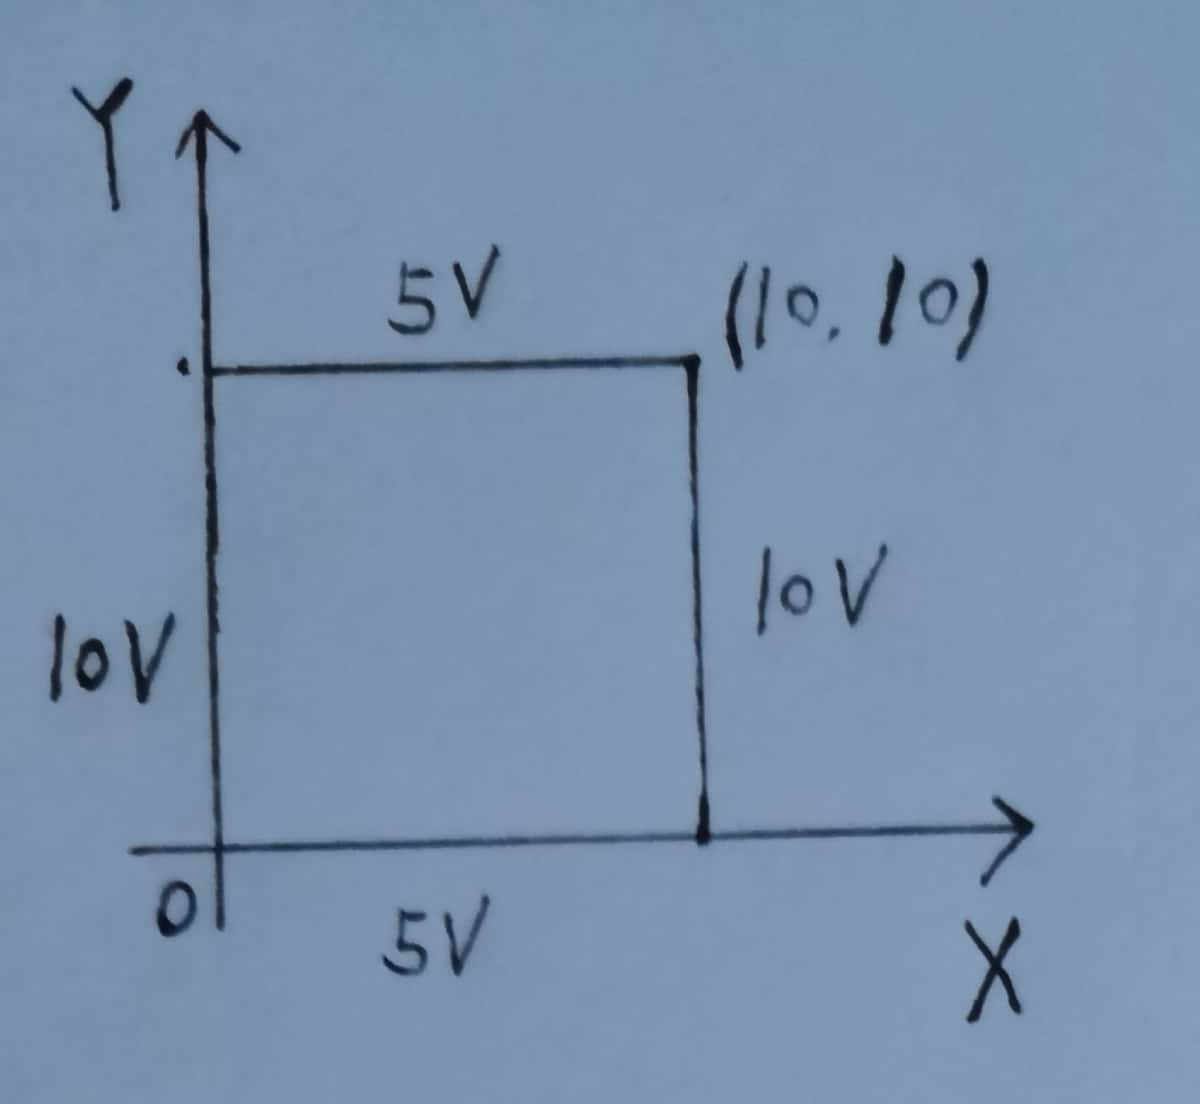
\includegraphics[width=3cm]{2015-1.jpg}
\end{wrapfigure}
\paragraph{}
一个二维正方形区域的静电场边界条件如右图。
\subsection{}
\paragraph{}
求区域内的电位分布$\varphi(x,y)$的解析表达式,通解的选取需要说明理由(10分)。
\subparagraph{解答}
\[\varphi=\varphi_1+\varphi_2+5\]
$\varphi_1$是左边界为5,其余为0的电势。$\varphi_2$是右边界为5,其余为0的电势。
\begin{equation*}
\begin{aligned}
&\varphi_1=\sum_n^{}A_nsin(\frac{n\pi}{10}y)sh(\frac{n\pi}{10}(10-x))\\
&\varphi_2=\sum_m^{}B_msin(\frac{n\pi}{10}y)sh(\frac{n\pi}{10}x)
\end{aligned}
\end{equation*}
其中$n=1,3,5,\cdots,m=1,3,5,\cdots$
\[\varphi=5+\varphi_1+\varphi_2\]
\subsection{}
\paragraph{}
在答题纸上(不是试卷)用虚线画出等位线。(5分)
\subsection{}
\paragraph{}
在答题纸上用实线画出电场线。(5分)
\begin{figure}[htbp]
\centering
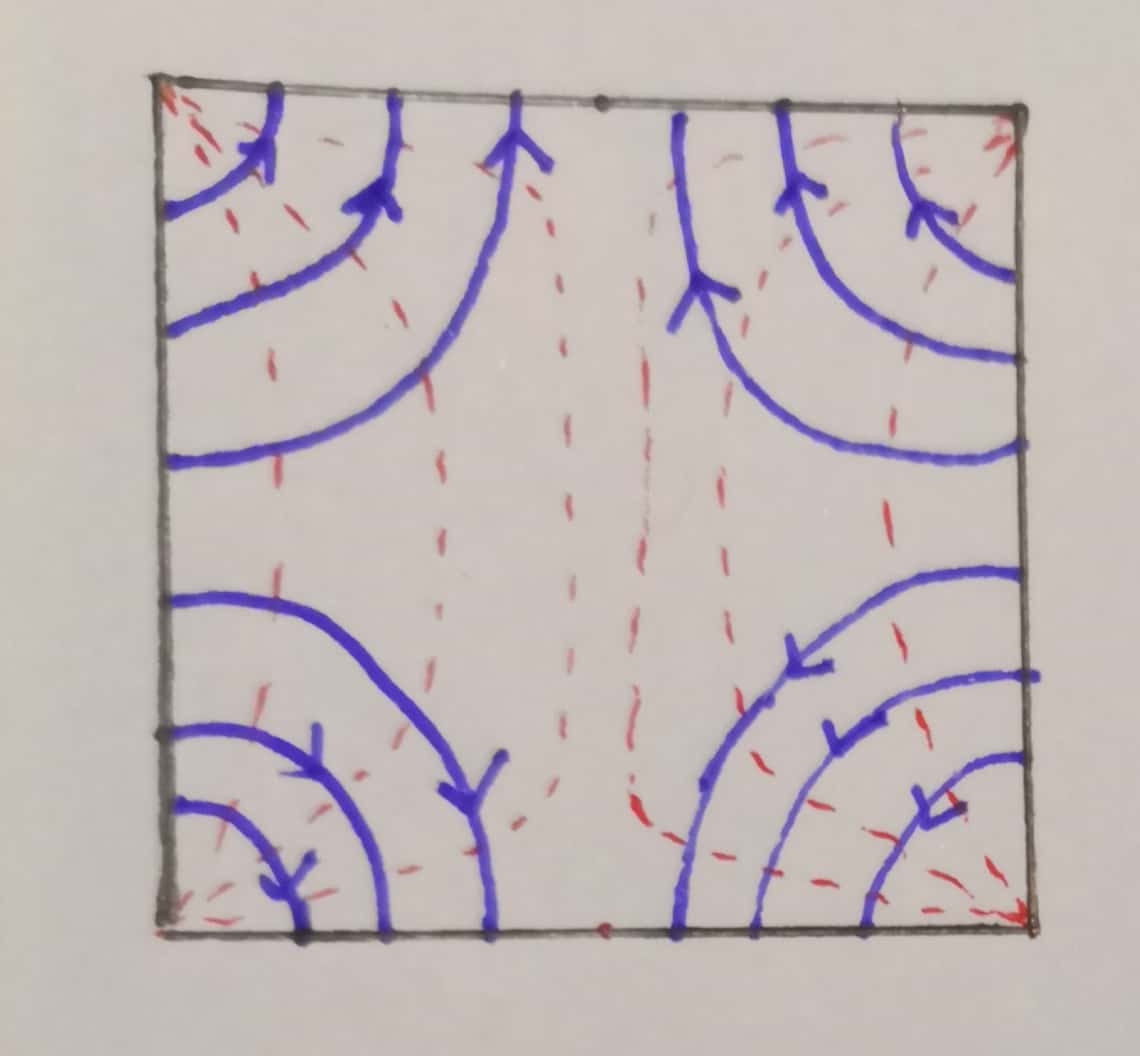
\includegraphics[width=3cm,height=3cm]{2015-2.jpg}
\end{figure}
\subsection{}
\paragraph{}
在0时刻,坐标(5,4)点上有一个静止的带正电荷的球,假设球和边界均为不形变的刚体,碰撞时不损失能量,请文字描述该球在0时刻过后的运动轨迹,不需要公式。(5分)
\subparagraph{解答}
先垂直下落,与边界碰撞后原速反弹,回到原点后停止,然后重复上述过程。
\section{}
\subsection{}
\paragraph{}
请写出理想导体矩形波导(尺寸40mm*30mm)截止频率最低的3个模式,并计算出它们各自的截止频率。(5分)
\subparagraph{解答}
\begin{equation*}
\begin{aligned}
&TE_{10}\\
&k^2=(\frac{2\pi}{\lambda})^2=(\frac{2\pi f}{c})^2=(\frac{\pi}{a})^2\\
&f=3.75GHz\\
&TE_{01}\\
&k^2=(\frac{2\pi}{\lambda})^2=(\frac{2\pi f}{c})^2=(\frac{\pi}{b})^2\\
&f=5GHz\\
&TE_{11}\\
&k^2=(\frac{\pi}{a})^2+(\frac{\pi}{b})^2\\
&f=12.5GHz
\end{aligned}
\end{equation*}
\subsection{}
\begin{wrapfigure}{r}{2cm}
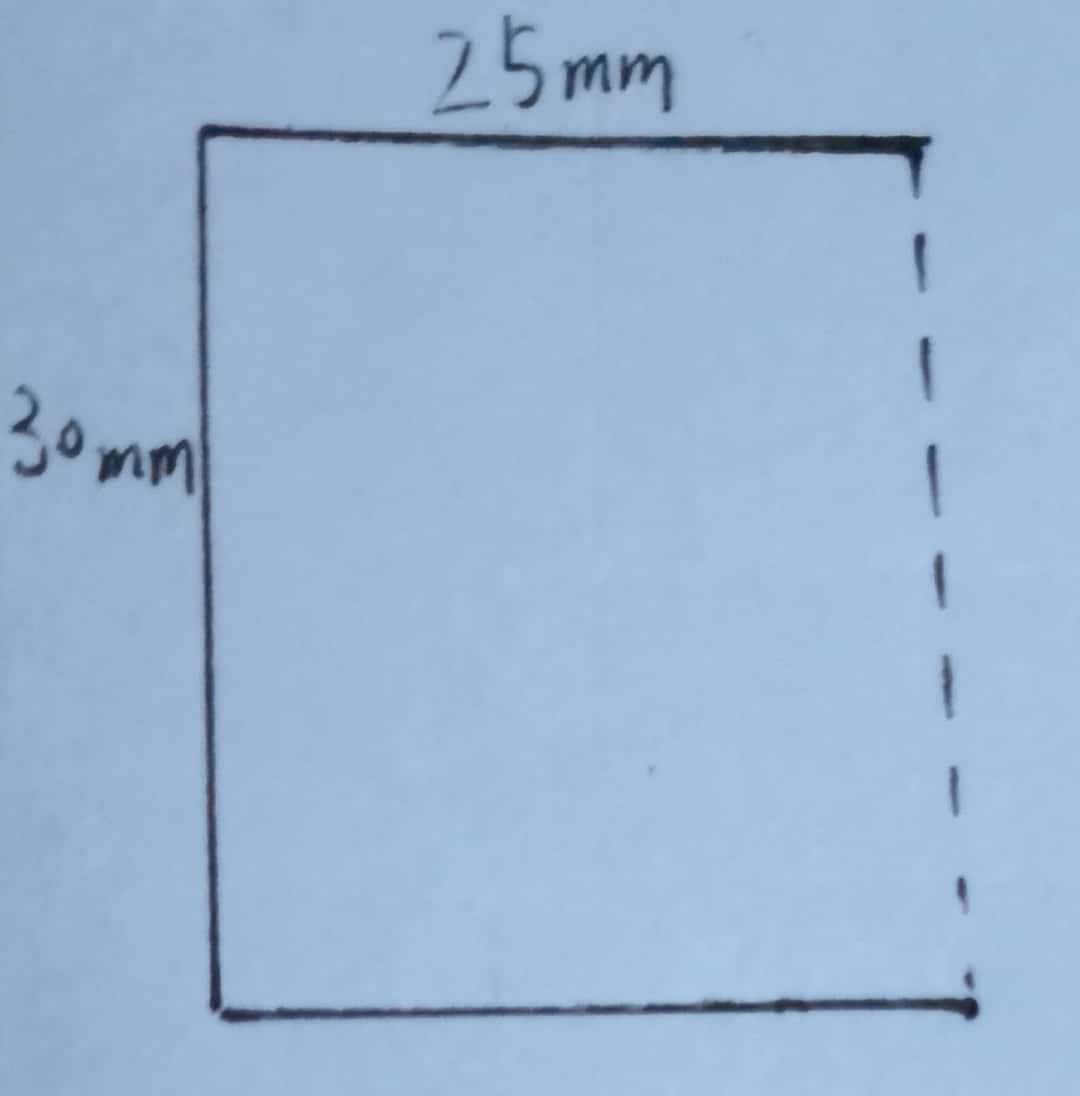
\includegraphics[width=2cm]{2015-3.jpg}
\end{wrapfigure}
\paragraph{}
请写出右图混合边界矩形波导(三个实线面为理想导体、电壁;虚线面为理想磁壁)可以传播的电磁波模式(TE?TM?TEM?)并说明为什么可以,为什么不可以。(5分)
\subparagraph{解答}
可以传TM和TE,不能传TEM。
\subsection{}
\paragraph{}
请计算该混合边界矩形波导最低截止频率。(5分)
\subparagraph{解答}
\begin{equation*}
\begin{aligned}
&\frac{\pi}{2X}=\frac{2\pi f}{c}\\
&f=3GHz
\end{aligned}
\end{equation*}
\subsection{}
\paragraph{}
请写出该混合边界矩形波导对应于最低截止频率的电场、磁场各分量的表达式(假设波导内场沿+Z方向传播,表达式中需要包含z的变化项,需要虚数符号j,不要求准确系数)。(5分)
\subparagraph{解答}
\begin{equation*}
\begin{aligned}
&a=50mm, b=30mm\\
&\vec E=\hat yjAsin(\frac{\pi}{a}x)e^{j(\omega t-kz)}\\
&\vec H=(\hat zBcos(\frac{\pi}{a}x)+\hat xCsin(\frac{\pi}{a}x))e^{j(\omega t-kz)}
\end{aligned}
\end{equation*}
\subsection{}
\paragraph{}
在答题纸上(不是试卷)画出该混合边界矩形波导对应于最低频率模式的三维电场(实线)的分布,三维磁场分布(虚线)。(5分)
\begin{figure}[htbp]
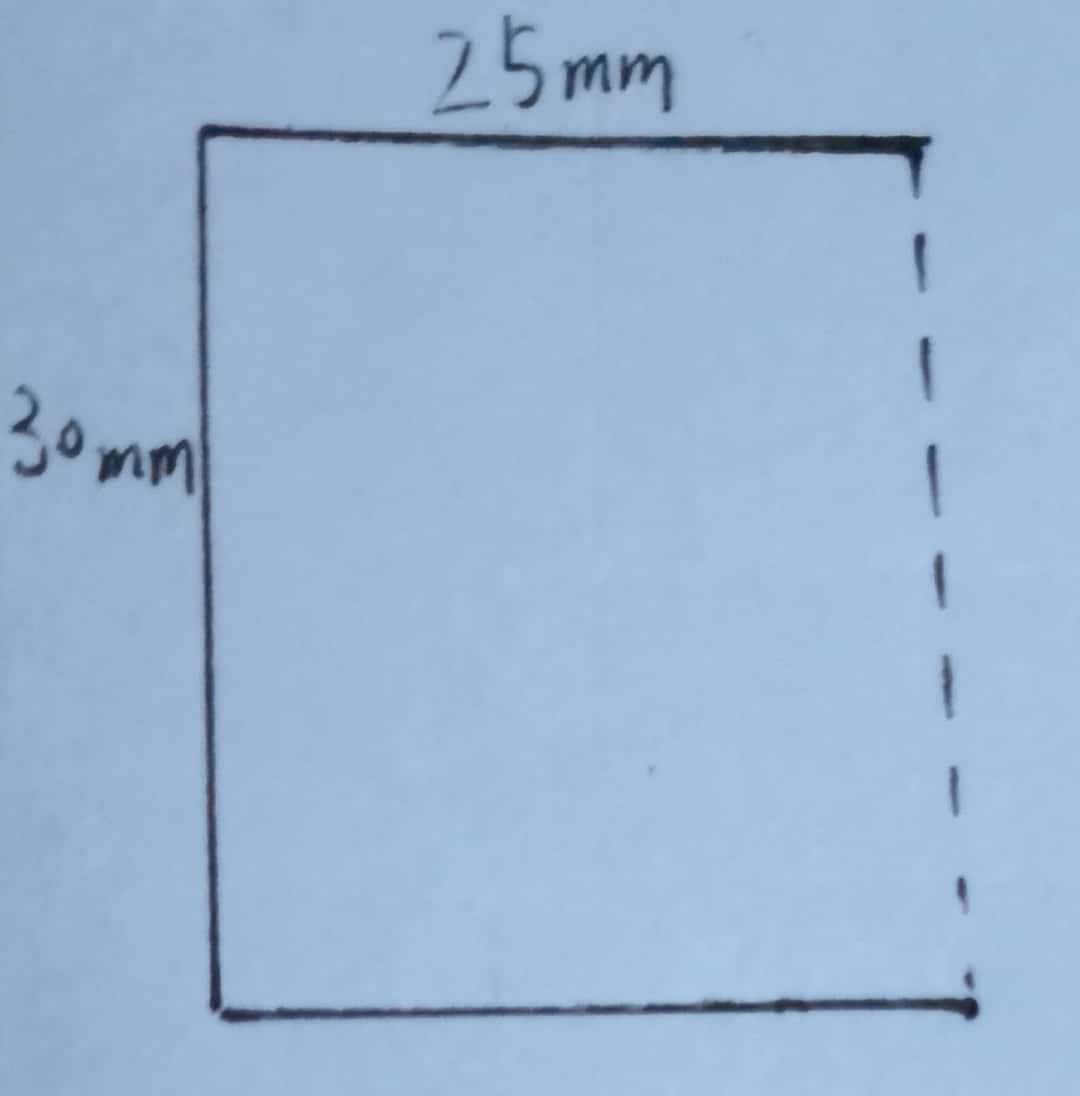
\includegraphics[width=4cm,height=3cm]{2015-3.jpg}
\centering
\end{figure}
\section{}
\begin{wrapfigure}{r}{3cm}
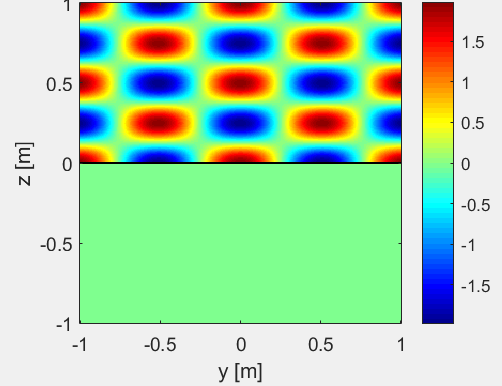
\includegraphics[width=3cm]{2015-4.png}
\end{wrapfigure}
\paragraph{}
已知z<0的空间为理想金属,全空间$\mu_r=1$。入射波的频率为300MHz,右图为yz平面内总场的场分布图。
\subsection{}
\paragraph{}
请问这是垂直极化波($E_x$)还是平行极化波($H_x$)?理由?(5分)\\
平行极化波。x方向的场在电壁上有切向分量,因此是磁场。
\subsection{}
\paragraph{}
假设波从左上角入射进来,求解入射波的k矢量。(5分)
\begin{equation*}
\begin{aligned}
&\lambda_z=0.5m,k_z=\frac{2\pi}{\lambda_z}\\
&\lambda_y=1m,k_y=\frac{2\pi}{\lambda_y}\\
&k=\sqrt{k_z^2 + k_y^2}=14.05
\end{aligned}
\end{equation*}
\subsection{}
\paragraph{}
求解介质的相对介电常数$\varepsilon_r$。(5分)
\begin{equation*}
\begin{aligned}
&k^2=\omega^2\mu \varepsilon=\omega^2\mu_0\varepsilon_r\varepsilon_0\\
&\varepsilon_r=\frac{k^2}{\omega^2\mu_0\varepsilon_0}=5
\end{aligned}
\end{equation*}
\subsection{}
\paragraph{}
请在答题纸上(不是试卷)画出电场图,要求在z,y方向上各画一个整周期($2\pi$)。(5分)
\begin{figure}[htbp]
\centering
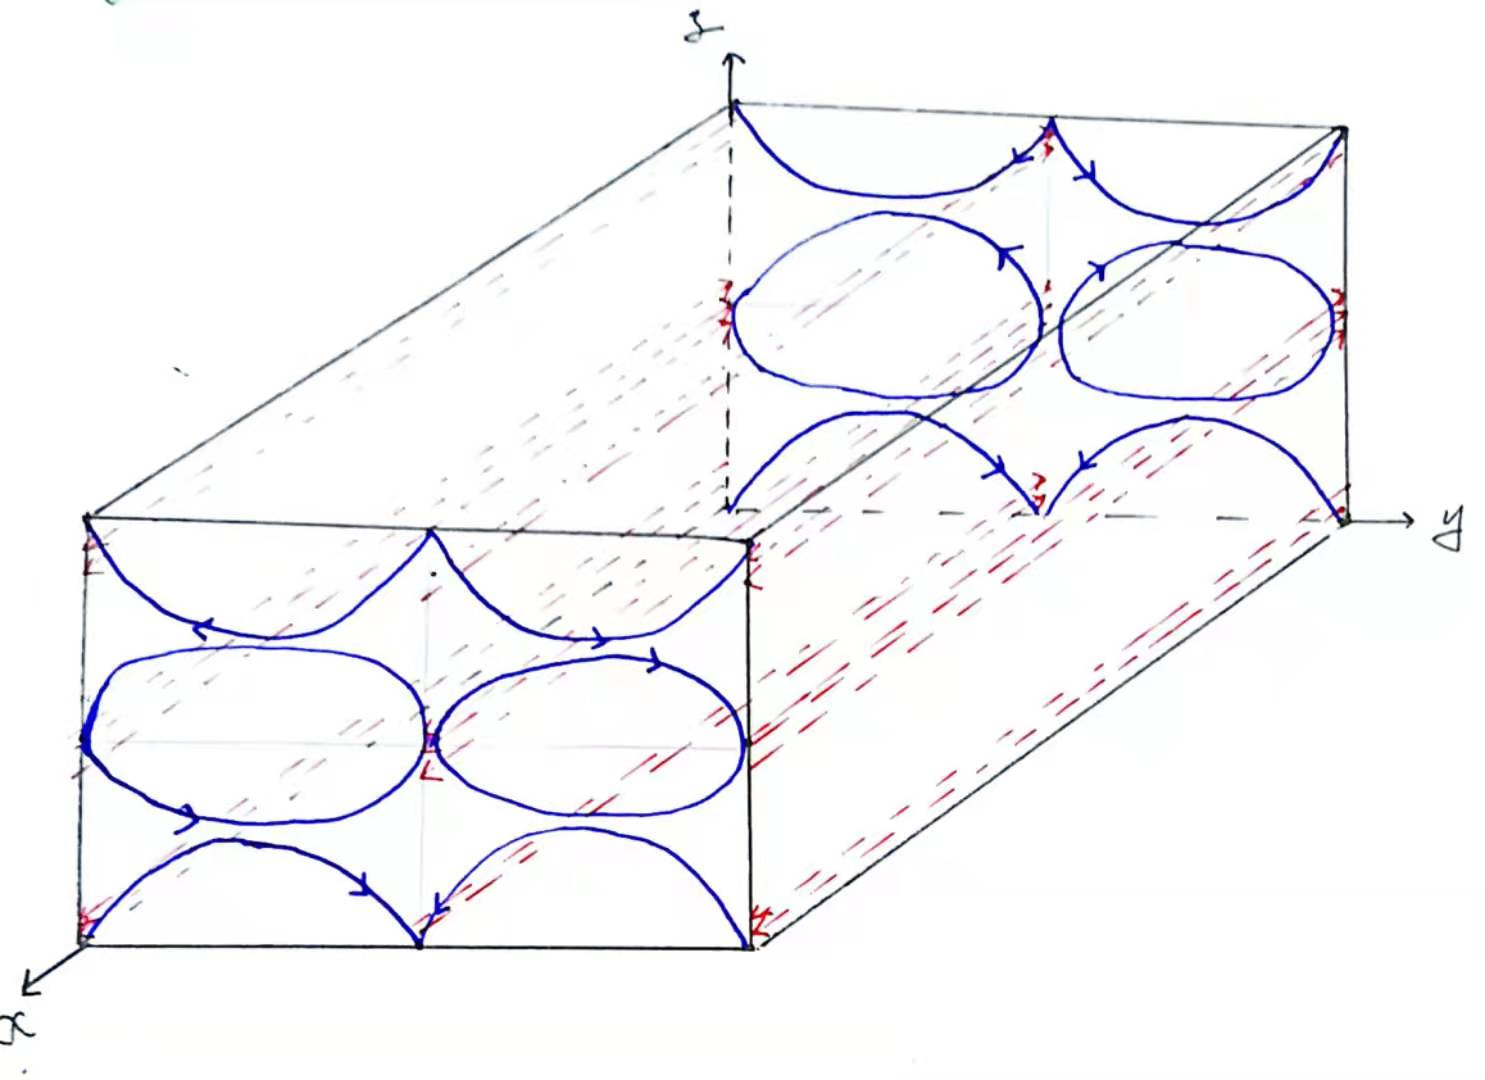
\includegraphics[width=4cm,height=3cm]{2015-4.jpg}
\end{figure}
\subsection{}
\paragraph{}
如果希望在z>0空间加一面无限大的理想导体平面,形成导波结构。加入后需保证z从0到0.4米的区域内,在传输相同频率的电磁波时,场型结构不变。请问理想导体表面可以加入的位置有哪些?(5分)\\
\[z=0.375+0.25n,\quad\quad n=1,2,3\cdots\]
\section{}
\paragraph{}
右图所示二维静电场问题中,X,Y正半轴上除虚线部分均满足$\frac{\partial\varphi(\vec r)}{\partial n}=0$。在X轴上[a,b]虚线区间内$\frac{\partial\varphi(\vec r)}{\partial n}=f(x)$,图中的灰色区域的电荷分布为g(x,y)。
\subsection{}
\paragraph{}
请给出本问题所对应的格林函数空间内的表达式G(x,y,x',y')=?(5分)
\[\nabla^2G(\vec r,\vec r')=-\delta(\vec r,\vec r')\]
\subsection{}
\paragraph{}
请问这是格林函数的第几类边值问题?请给出该格林函数G的边界条件。(5分)
\[\frac{\partial G}{\partial y}\lvert_{y=0}=0, G\lvert_{x=0}=0\]
第一类边值问题。
\subsection{}
\paragraph{}
请给出本问题化简后电势的积分形式格林函数表达式。$\varphi(\vec r)=$?(5分)
\[\varphi(\vec r)=\int_S^{}{\frac{\rho G}{\varepsilon}dS}-\int_a^b{f(x)G}\]
其中S是g(x,y)存在的区域。
\subsection{}
\paragraph{}
请给出该格林函数的解析解$G(\vec r,\vec r')$。(提示:二维问题,通解ln)(5分)
\begin{equation*}
\begin{aligned}
&G(\vec r,\vec r')=\frac{1}{2\pi}ln(\frac{1}{r_1r_2r_3r_4})\\
&r_1=\sqrt{(x-x')^2+(y-y')^2}\\
&r_2=\sqrt{(x+x')^2+(y-y')^2}\\
&r_3=\sqrt{(x+x')^2+(y+y')^2}\\
&r_4=\sqrt{(x-x')^2+(y+y')^2}
\end{aligned}
\end{equation*}
\subsection{}
\paragraph{}
假定源点位于(x',y'),在答题纸上(不是试卷)画出该格林函数的电场(实线)、等位线(虚线)。(5分)
\begin{figure}[H]
\centering
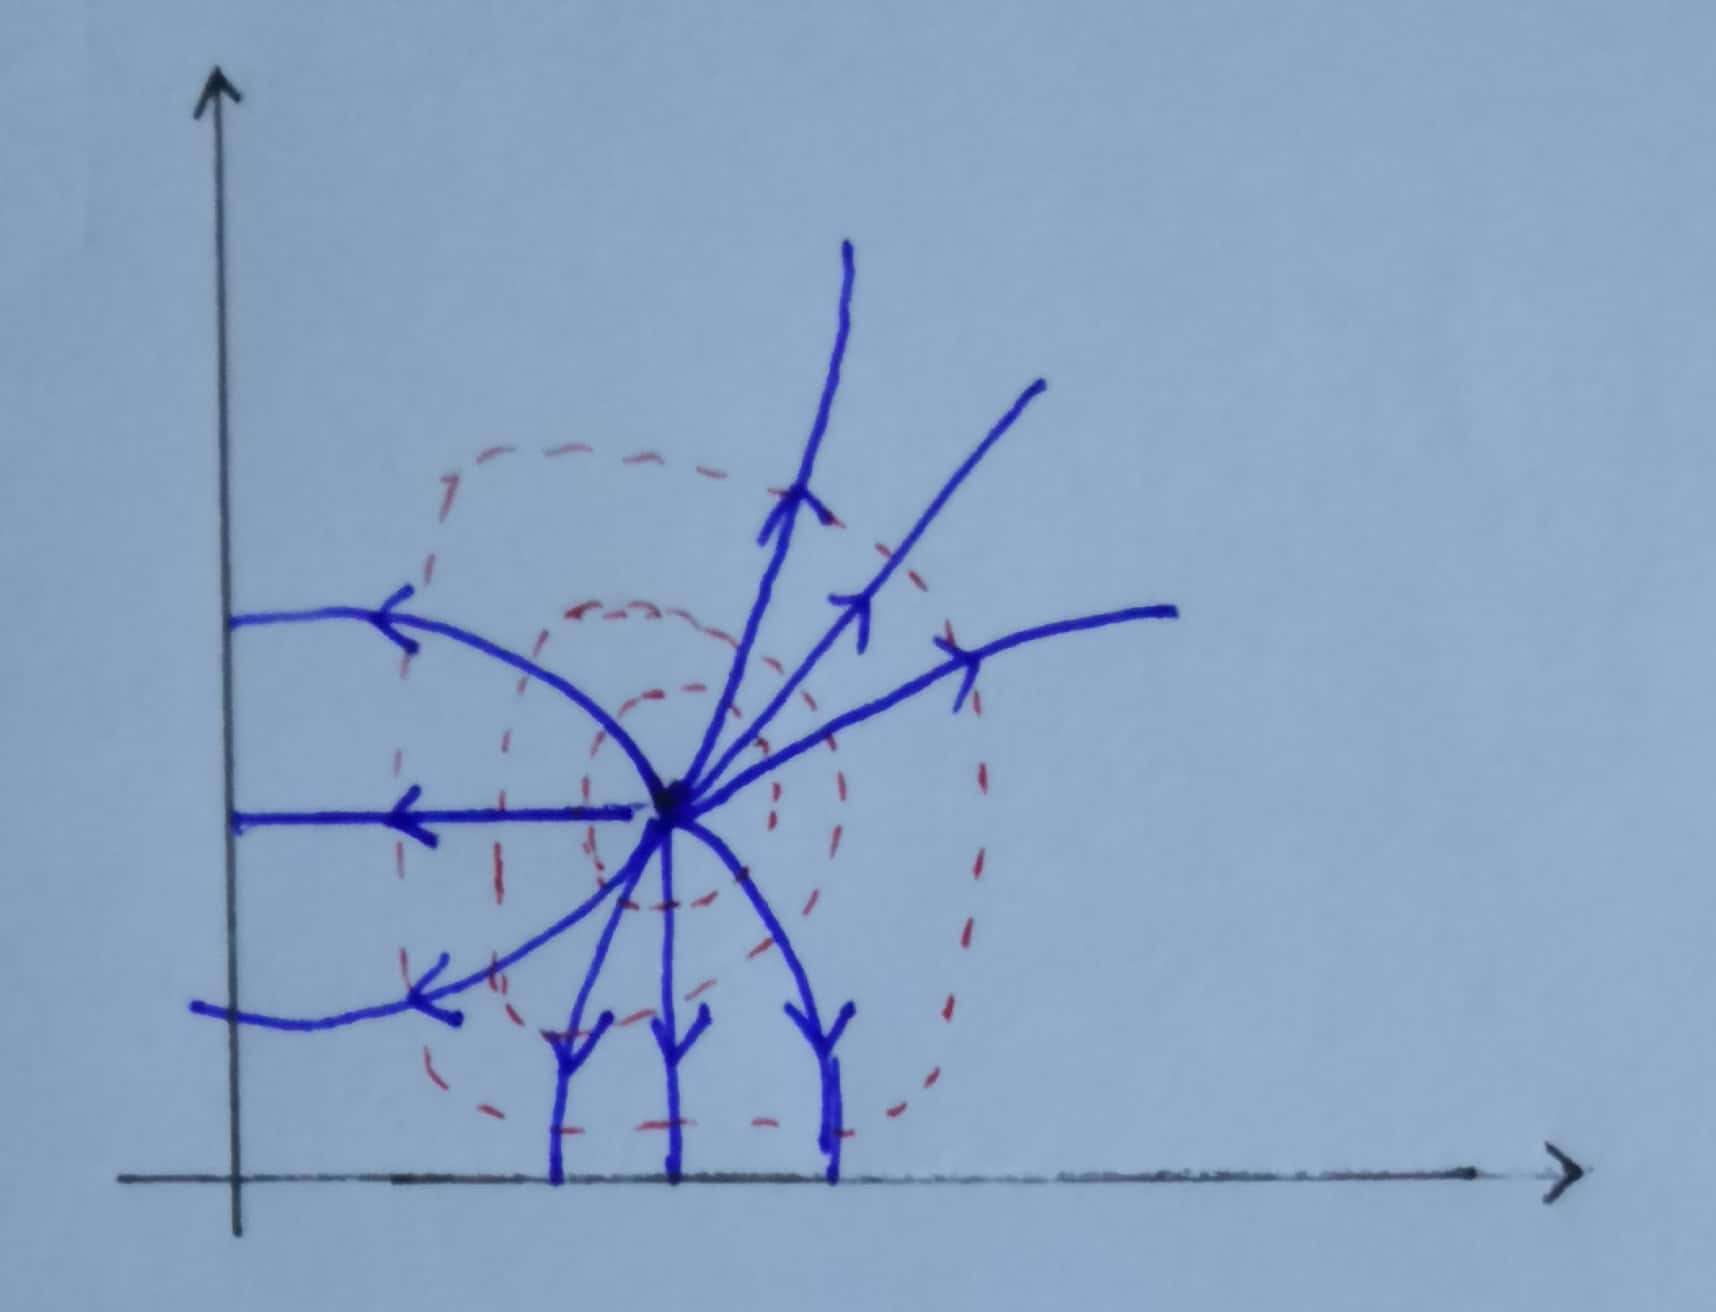
\includegraphics[width=6cm,height=4cm]{2015-5.jpg}
\end{figure}
\end{document}
